

\section{Design} \label{sec:design} 

% In this section, we synthesize requirements and design the architectures of two models of different architectural complexities.

In this section, we synthesize requirements and design two models of opposite architectural complexities.



\begin{figure*}
    \centering
    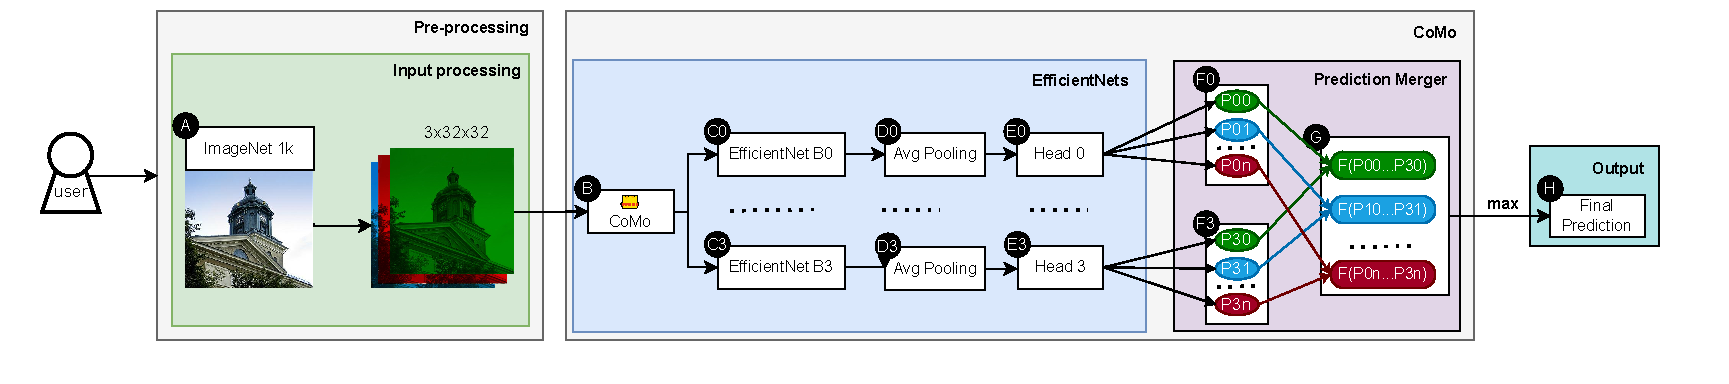
\includegraphics[width=0.95\linewidth]{figures/design-como.pdf}
    \caption{A high-level architectural overview of CoMo, a complex architectural model.}
    \label{fig:design:como}
\end{figure*}

\subsection{Requirement Analysis} \label{sec:m3sa:requirements-analysis}
%\begin{enumerate}[label=\textbf{(FR\arabic*)}, leftmargin=3em]
\begin{enumerate}[label=\textbf{(FR\arabic*)}, leftmargin=0pt, itemindent=3em]
    \item \label{fr1} \textbf{\underline{Si}mple architectural \underline{Mo}del for object classification} This research should involve a simple architectural model, the SiMo model. Despite the inherent simplicity, SiMo should be able to conduct object classification, while still meeting the other functional and non-functional requirements.
    
    \item \label{fr2} \textbf{\underline{Co}mplex architectural \underline{Mo}del for object classification}: 
    This research should involve a complex architectural model, CoMo, able to conduct object classification. CoMo should predict using under the hood multiple open-source, peer-reviewed, and community-vetted models, and integrate their predictions into a final prediction, thus filtering individual model biases, and enhancing prediction reliability.    

    \item \label{fr3} \textbf{Open-source and reproducible}: 
    Data created and used in this work should be open-sourced, following the principles of open science. Experiments should be reproducible.
\end{enumerate}

\begin{enumerate}[label=\textbf{(NFR\arabic*)}, leftmargin=0pt, itemindent=3em]
    \item \label{nfr1} \textbf{Provide live, instantaneous predictions}: 
    Both SiMo and CoMo should be able to classify first-time-seen, individual objects under 2 seconds. The models should be able to each predict batches of 100 images under 1 minute.
    
    \item \label{nfr2} \textbf{Highly accurate predictions}: 
    Models' accuracy should be at least 8 times higher than the guessing factor (e.g., for 16 classes the guessing factor is $6.25\%$; models'  accuracy should be at least $ 8\cdot6.25\%$).
    
    \item \label{nfr3} \textbf{Leverage four, peer-reviewed, community-vetted models}: 
    CoMo should employ four peer-reviewed and community-vetted individual models, and leverage their predictions into an atomic prediction.

    \item \label{nfr4} \textbf{Multiple-class operability}: 
    CoMo and SiMo should predict at least 16 classes of objects. This limited and computer science round number, should serve as a proof of concept, and suffice the research and experimental basis of this work.

    \item \label{nfr5} \textbf{Limited resources operability}: 
    Training and inference should be conducted on a small-sized cluster (i.e., not a supercomputer), while still meeting all the aforementioned requirements.

    
\end{enumerate}


\subsection{Design of SiMo, a \underline{Si}mple architectural \underline{Mo}del}\label{sec:design:simo}

SiMo (Simple architectural Model) architecture is designed to provide a straightforward yet effective solution for object classification tasks. The term ``simple" refers to SiMo's relative simplicity in comparison to more complex models while still being sufficiently sophisticated to meet the functional and non-functional requirements\ref{fr1}. For this purpose, SiMo employs a 3-layer convolutional neural network (CNN), providing a balance between depth and efficiency and ensuring that the model captures complex patterns without excessive computational costs.

We train, validate and test SiMo on Imagenet-1k \cite{DBLP:conf/cvpr/DengDSLL009}, a large scale dataset commonly used for benchmarking and consisting of 1000 classes, thus ensuring SiMo fulfills \ref{nfr4}.

Figure \ref{fig:design:f3} depicts a high-level overview of SiMo. The process of SiMo begins in step \circled{A}. After data pre-processing (further expanded in \Cref{sec:implementation}), the input image is fed into the network. The network itself consists of three convolutional layers (\circled{B1}-\circled{B3}), each progressively increasing the number of output nodes (\circled{B1} contains 64 output nodes, \circled{B2} contains 128 output nodes, \circled{B3} contains 256 output nodes). This simple yet powerful design choice allows the network to capture a wide range of features, from simple patterns in early layers to more complex representations in the deeper ones \ref{nfr2}. We apply batch normalization after each convolution to stabilize training and keep values in the network within a reasonable range \cite{NEURIPS2018_905056c1}. We use ReLU activation to introduce non-linearity as it is a standard practice in neural networks \cite{rasamoelina2020review}. 

Furthermore, this design utilizes 5x5 MaxPooling after each convolutional layer to reduce the spatial dimensions of the feature maps, increasing the model's efficiency by reducing complexity while still preserving the main information needed for accurate predictions.

Unlike deeper architectures, SiMo does not include dropout, as its shallow design inherently limits overfitting. Overfitting is a concern in deeper networks with millions of parameters, but SiMo’s simplicity naturally mitigates this risk. Adding dropout would introduce unnecessary stochastic operations, slowing down both training and inference \ref{nfr1} without providing meaningful gains in accuracy or generalization \ref{nfr2}.

Lastly, after passing through the convolutional layers, the output is flattened and passed to a fully connected layer \circled{C} with 1000 output units, corresponding to the number of classes and ensuring \ref{nfr4} is met, which performs the classification in step~\circled{D}. This final layer ensures that SiMo remains lightweight and efficient \ref{nfr1}. 

This overall design choice, with the high-level picture depicted in \Cref{fig:design:simo}, allows SiMo to strike a robust balance between simplicity and performance, making the model well-suited for object classification tasks where computational resources are limited. In \Cref{sec:experiments}, we analyze the performance of SiMo prototype embodying the architecture depicted in \Cref{fig:design:simo}, and able to predict 1,000 classes. We measure an accuracy of 34.37\%, and the ability to run on average 5795.5 samples per second.



% ==================================================================================================================



\subsection{Design of CoMo, a \underline{Co}mplex architectural \underline{Mo}del}\label{sec:design:como}

CoMo, a Complex Architectural Model, is designed for highly accurate object detection despite posing an inherent complexity \ref{fr2}. \Cref{fig:design:como} depicts an overview of CoMo architecture, in which CoMo embeds four versions of EfficientNet \cite{tan_efficientnet_2020}, a vetted, state-of-the-art, and widely used family of models, with proven accuracy and performance on datasets as CIFAR-100 or Flower~\cite{DBLP:conf/icml/TanL19}. We train, validate, and test the CoMo using ImageNet-1k\cite{DBLP:conf/cvpr/DengDSLL009}, a large-scale dataset, with 1,000 classes, thus ensuring the multiple-class operability of CoMo \ref{nfr4}.

We design CoMo as able to integrate versions B0, B1, B2, and B3 of the EfficinetNet family \ref{nfr3}, yet design and engineer CoMo as simply expandable to higher iterations of the EfficientNet. This design serves as a proof of concept that is especially relevant for testing out prototypes of financially costly machine learning applications. We archive our design goals by building CoMo under limited computation resource availiable; we argue that, albeit valuable for CoMo to include up to iteration B8, such a design would result in an unfeasible model for the limitations of this research. We thus regard B0-B4 as sufficient to meet complexity requirements \ref{fr2}, model multiplicity \ref{nfr3}, and accuracy requirements \ref{nfr2} while still meeting the requirement of limited resources operability \ref{nfr5}.

\textit{Input processing step:} The CoMo process begins in step~\circled{A}, with an image provided by the user, e.g., an image from the test split of ImageNet-1k. The image undergoes pre-processing and resides in a three-dimensional tensor of size 3x32x32, thus ensuring uniformity across inputs and compatibility with the EfficientNet models. The processed input is then fed into CoMo (\circled{B}).

\textit{EfficientNets step:} CoMo underlies four versions of EfficientNet, run in parallel, and each sub-model predicts without interfering with one another~\ref{fr2}. Besides, each submodel underlies an identical architecture and has a single differing element, the version of the EfficientNet (\circled{C0} - \circled{C3}); thus, to prevent redundancy, we will further detail only the submodel using EfficientNet B0. The predictions B0 are fed into an average pooling layer (\circled{D0}), which compresses the spatial information into a fixed-length vector by averaging the values in each feature to produce a single value per channel. Further, the input is fed into a head (\circled{E0}), which flattens the pooling layer and classifies the image, thus preparing predictions for the aggregation step.

\textit{Prediction aggregation step:} The prediction merger component is designed to maximize accuracy \ref{nfr2} by alleviating individual model biases and filtering out extremes, thus strengthening prediction robustness. In elements~\circled{F0} - \circled{F3}, the system leverages predictions of each submodel per each class. \Cref{fig:design:como} labels the predictions following the structure P[model id][class id] (e.g., P01 represents class 1 of model 0). The leveraged predictions are further fed into an aggregation function, which combines the predictions (\circled{G}). After applying the aggregation function, the class with the highest probability is selected as the final prediction and delivered as the output of the system (\circled{H}).

Choosing an aggregation function for element \circled{G} is a non-trivial process that needs to address the accuracy complexity trade-off.
The function used in \circled{G} could be either a statistical function (e.g., mean, median) or ML-based. We further analyze the benefits of each approach. Firstly, statistical functions could be a computational light approach, with (arithmetic) \textit{mean} used for aggregating predictions in datacenter simulation~\cite{nicolae2025m3sa}, ecology~\cite{harrison2018brief}, and meteorology~\cite{myhre2017multi}, but has a high sensitivity to outliers, and \textit{median}, which alleviates the outlier sensitivity of the mean but is more computationally expensive~\cite{nicolae2025m3sa}. Secondly, ML-based aggregation functions would add extra complexity and computation time, which would hinder and bias the performance and accuracy comparison between the core architectures of SiMo, a model comprising only three hidden layers, and CoMo, a model embodying four large-scale pre-trained models; an additional heavy-weight computation in the aggregation component could improve the overall accuracy \ref{nfr2}, but bias the measurements from \Cref{sec:experiments}, thus deviating from the original purpose of \ref{introduction:mrq}. We, therefore, choose the statistical approach and combine predictions using (arithmetic) mean.  

These design choices, synthesized into the high-level architecture from \Cref{fig:design:como}, allow CoMo to balance complexity with performance and accuracy. In \Cref{sec:experiments}, we analyze the performance of a CoMo prototype embodying the architecture described in this section and are able to predict for 1,000 classes; we further compare CoMo with SiMo on various metrics. We quantify CoMo and obtain an accuracy of 57.8\% and the ability to run on average 321.63 samples per second. The measured throughput (samples/sec) for mile-predictions of SiMo is 18 times bigger than that of CoMo.
